\documentclass[11pt,a4paper]{scrartcl}
% =====================================================================
%  pds-apuntes.tex — Estilo común de apuntes y hojas de ejercicios.
%
%  Uso (desde teoría/Tx/apuntes/ o teoría/Tx/ejercicios/):
%     \documentclass[11pt,a4paper]{scrartcl}   % o scrreprt
%     % =====================================================================
%  pds-apuntes.tex — Estilo común de apuntes y hojas de ejercicios.
%
%  Uso (desde teoría/Tx/apuntes/ o teoría/Tx/ejercicios/):
%     \documentclass[11pt,a4paper]{scrartcl}   % o scrreprt
%     % =====================================================================
%  pds-apuntes.tex — Estilo común de apuntes y hojas de ejercicios.
%
%  Uso (desde teoría/Tx/apuntes/ o teoría/Tx/ejercicios/):
%     \documentclass[11pt,a4paper]{scrartcl}   % o scrreprt
%     \input{../../comun/pds-apuntes}
%     \tema{1}{Introducción: señales y sistemas}
%     \begin{document} \cabecera{Apuntes} ... \end{document}
%  Compilar con:  latexmk -xelatex  (o «make» desde teoría/)
% =====================================================================

\input{../../comun/pds-comun.tex}

\usepackage[a4paper, top=2.6cm, bottom=2.6cm, left=2.5cm, right=2.5cm,
            headheight=1.1cm]{geometry}
\usepackage{fontspec}
\usepackage{unicode-math}
\setmainfont{LibertinusSerif}[Extension=.otf, UprightFont=*-Regular, BoldFont=*-Semibold,
  ItalicFont=*-Italic, BoldItalicFont=*-SemiboldItalic]
\setsansfont{FiraSans}[Extension=.otf, UprightFont=*-Regular, BoldFont=*-SemiBold,
  ItalicFont=*-Italic, BoldItalicFont=*-SemiBoldItalic, Scale=MatchLowercase]
\setmonofont{FiraMono}[Extension=.otf, UprightFont=*-Regular, BoldFont=*-Medium, AutoFakeSlant=0.15, Scale=0.85]
\setmathfont{LibertinusMath-Regular.otf}

\usepackage{microtype}
\usepackage{enumitem}
\usepackage{multicol}
\setlist{itemsep=2pt, topsep=4pt}
\usepackage{caption}
\captionsetup{font=small, labelfont={sf,bf,color=pdsazul}, labelsep=period}
\usepackage{subcaption}
\usepackage[most]{tcolorbox}
\usepackage{environ}
\usepackage{scrlayer-scrpage}
\usepackage[hidelinks, unicode]{hyperref}
\usepackage[spanish, noabbrev]{cleveref}

% Títulos en Fira Sans con el azul de la asignatura
\setkomafont{disposition}{\sffamily\bfseries\color{pdsazul}}
\setkomafont{descriptionlabel}{\sffamily\bfseries}
\setlength{\parindent}{0pt}
\setlength{\parskip}{0.55\baselineskip plus 2pt}
\linespread{1.05}

% ---------------------------------------------------------------------
%  Datos del tema y cabeceras
% ---------------------------------------------------------------------
\newcommand{\numtema}{}
\newcommand{\nombretema}{}
\newcommand{\tema}[2]{\renewcommand{\numtema}{#1}\renewcommand{\nombretema}{#2}}

\pagestyle{scrheadings}
\clearpairofpagestyles
\ihead{\sffamily\small\color{pdsgris}\asignatura}
\ohead{\sffamily\small\color{pdsgris}Tema~\numtema. \nombretema}
\ifoot{\sffamily\small\color{pdsgris}\grado}
\ofoot{\sffamily\small\pagemark}
\setkomafont{pagehead}{\normalfont}
\setkomafont{pagefoot}{\normalfont}

% \cabecera{Apuntes|Ejercicios|...} : bloque de título de la primera página
\newcommand{\cabecera}[1]{%
  \thispagestyle{plain.scrheadings}%
  \noindent
  \begin{minipage}[c]{2.2cm}
    
\includegraphics[width=1.9cm]{../../comun/ucm.png}
  \end{minipage}%
  \begin{minipage}[c]{\dimexpr\linewidth-2.2cm}
    \sffamily
    {\small\color{pdsgris}\grado\par \asignatura\ · \curso\par}
    \vspace{4pt}
    {\Large\bfseries\color{pdsazul}#1\par}
    {\large\bfseries Tema~\numtema. \nombretema\par}
    \vspace{2pt}
    {\small\color{pdsgris}\autores\par}
  \end{minipage}\par
  \vspace{6pt}{\color{pdsazul}\rule{\linewidth}{0.8pt}}\par\vspace{4pt}}

% ---------------------------------------------------------------------
%  Cajas: definición, propiedad, ejemplo, nota, «en código»
% ---------------------------------------------------------------------
\tcbset{pdsbase/.style={enhanced, breakable, boxrule=0pt, arc=1.5pt, left=8pt, right=8pt,
    top=5pt, bottom=5pt, fonttitle=\sffamily\bfseries\small, coltitle=white,
    before skip=8pt, after skip=8pt}}
\newtcbtheorem[number within=section]{definicion}{Definición}%
  {pdsbase, colback=pdsfondo, colframe=pdsazul, borderline west={2.5pt}{0pt}{pdsazul}}{def}
\newtcbtheorem[use counter from=definicion]{propiedad}{Propiedad}%
  {pdsbase, colback=pdsfondo, colframe=pdsazul!75, borderline west={2.5pt}{0pt}{pdsazul!75}}{prop}
\newtcbtheorem[use counter from=definicion]{ejemplo}{Ejemplo}%
  {pdsbase, colback=pdsverde!5, colframe=pdsverde, borderline west={2.5pt}{0pt}{pdsverde}}{ej}
\newtcolorbox{nota}[1][Nota]{pdsbase, colback=pdsnaranja!7, colframe=pdsnaranja,
  title={#1}, borderline west={2.5pt}{0pt}{pdsnaranja}}
\newtcolorbox{importante}[1][Importante]{pdsbase, colback=pdsrojo!5, colframe=pdsrojo,
  title={#1}, borderline west={2.5pt}{0pt}{pdsrojo}}
\newtcolorbox{encodigo}[1][En código]{pdsbase, colback=white, colframe=pdsgris,
  title={#1}, borderline west={2.5pt}{0pt}{pdsgris}}

\lstset{basicstyle=\ttfamily\small}
\renewcommand{\codigoetiqueta}[1]{{\sffamily\small\bfseries\color{pdsgris}#1}}

% ---------------------------------------------------------------------
%  Hojas de ejercicios: \begin{ejercicio} ... \end{ejercicio} y
%  \begin{solucion} ... \end{solucion} (solo se imprime si se define
%  \SOLUCIONES antes de cargar el documento; ver *-Soluciones.tex)
% ---------------------------------------------------------------------
\newif\ifsoluciones
\ifdefined\SOLUCIONES \solucionestrue \fi
\newcounter{ejercicio}
\newenvironment{ejercicio}[1][]{%
  \refstepcounter{ejercicio}\par\vspace{6pt}%
  \noindent{\sffamily\bfseries\color{pdsazul}Ejercicio~\theejercicio}%
  \if\relax\detokenize{#1}\relax\else\ {\sffamily\color{pdsgris}(#1)}\fi\quad}%
  {\par}
\NewEnviron{solucion}{%
  \ifsoluciones
    \begin{tcolorbox}[pdsbase, colback=pdsverde!4, colframe=pdsverde,
      borderline west={2.5pt}{0pt}{pdsverde}, title={Solución}]
      \BODY
    \end{tcolorbox}
  \fi}
% \begin{incisos}[columnas] ... \end{incisos}: apartados a), b)... de un
% enunciado repartidos en columnas (3 por defecto)
% (con una sola columna no se usa multicols, que necesita al menos dos)
\newenvironment{incisos}[1][3]{\par\vspace{-2pt}%
  \ifnum#1>1 \def\finincisos{\end{multicols}}\begin{multicols}{#1}\raggedcolumns\raggedright
  \else\def\finincisos{}\fi
  \begin{enumerate}[label=\alph*), itemsep=3pt, topsep=0pt]}%
  {\end{enumerate}\finincisos\vspace{-4pt}}
\newcommand{\herramienta}[1]{\emph{Herramienta interactiva:} \texttt{herramientas/#1}}

%     \tema{1}{Introducción: señales y sistemas}
%     \begin{document} \cabecera{Apuntes} ... \end{document}
%  Compilar con:  latexmk -xelatex  (o «make» desde teoría/)
% =====================================================================

% =====================================================================
%  pds-comun.tex — Paquetes, colores y estilos de código comunes a
%  transparencias, apuntes y hojas de ejercicios. Compilar con XeLaTeX.
%  No cargar directamente: lo cargan pds-beamer.tex y pds-apuntes.tex.
% =====================================================================

\usepackage{polyglossia}
\setmainlanguage{spanish}
\usepackage{mathtools}
\usepackage{graphicx}
\usepackage{booktabs}
\usepackage{multirow}
\usepackage{array}
\usepackage{xcolor}
\usepackage{tikz}
\usetikzlibrary{positioning,arrows.meta,calc,shapes.geometric,decorations.pathreplacing}
\usepackage{listings}
\usepackage{siunitx}
\sisetup{output-decimal-marker={,}, group-separator={\,}, per-mode=symbol}

% Notas de erratas de versiones anteriores: no se imprimen salvo que se
% defina \ERRATAS antes de cargar el estilo (make ERRATAS=1)
\newif\iferratas
\ifdefined\ERRATAS \erratastrue \fi

% Ruta común (logo y figuras compartidas)
\providecommand{\rutacomun}{../../comun/}
\input{\rutacomun datos.tex}

% ---------------------------------------------------------------------
%  Paleta (la misma que usan las figuras generadas con Python,
%  ver comun/pds_estilo.py)
% ---------------------------------------------------------------------
\definecolor{pdsazul}{HTML}{2B3A8C}
\definecolor{pdsrojo}{HTML}{C0392B}
\definecolor{pdsverde}{HTML}{1E7B4F}
\definecolor{pdsnaranja}{HTML}{D9822B}
\definecolor{pdsgris}{HTML}{5A5A66}
\definecolor{pdsfondo}{HTML}{F3F4FA}
\definecolor{pdscodigo}{HTML}{F7F7F2}

% ---------------------------------------------------------------------
%  Diagramas de bloques (TikZ)
% ---------------------------------------------------------------------
\tikzset{
  bloque/.style={rectangle, rounded corners=2pt, draw=pdsazul!80, fill=pdsfondo,
                 very thick, minimum height=8mm, minimum width=14mm, align=center},
  sumador/.style={circle, draw=pdsazul!80, fill=pdsfondo, thick, inner sep=1.5pt},
  flecha/.style={-{Stealth[length=2.2mm]}, thick, pdsgris},
}

% ---------------------------------------------------------------------
%  Código: Python y Matlab en paralelo
% ---------------------------------------------------------------------
\newcommand{\pdscodesize}{\footnotesize}
\lstdefinestyle{pds}{
  basicstyle=\ttfamily\pdscodesize,
  keywordstyle=\color{pdsazul}\bfseries,
  commentstyle=\color{pdsverde}\itshape,
  stringstyle=\color{pdsrojo},
  numbers=none,
  backgroundcolor=\color{pdscodigo},
  frame=single, rulecolor=\color{pdsgris!40}, framerule=0.4pt,
  xleftmargin=2pt, xrightmargin=2pt, aboveskip=2pt, belowskip=2pt,
  columns=fullflexible, keepspaces=true,
  showstringspaces=false, breaklines=true, tabsize=4,
  upquote=true,
  % Con XeLaTeX, listings desordena los caracteres no ASCII junto a
  % dígitos («2π» sale «π2»): se sustituyen por su versión matemática.
  literate={π}{{$\pi$}}1 {δ}{{$\delta$}}1 {ω}{{$\omega$}}1 {Ω}{{$\Omega$}}1
           {≈}{{$\approx$}}1 {µ}{{$\mu$}}1 {·}{{$\cdot$}}1 {α}{{$\alpha$}}1
           {á}{{á}}1 {é}{{é}}1 {í}{{í}}1 {ó}{{ó}}1 {ú}{{ú}}1 {ñ}{{ñ}}1 {¿}{{¿}}1,
}
\lstdefinestyle{python}{style=pds, language=Python,
  morekeywords={as,True,False,None}}
\lstdefinestyle{matlab}{style=pds, language=Matlab,
  morekeywords={function,end,true,false}}

% \codigo{<ruta sin extensión>} muestra el mismo ejemplo en Python
% y en Matlab, uno al lado del otro. Los ficheros viven en
% ../codigo/python/<nombre>.py y ../codigo/matlab/<nombre>.m y se
% ejecutan en las pruebas (make prueba-codigo).
\newcommand{\rutacodigo}{../codigo/}
\newcommand{\codigoetiqueta}[1]{{\sffamily\scriptsize\bfseries\color{pdsgris}#1}}
\newcommand{\codigo}[2][]{%
  \par\noindent
  \begin{minipage}[t]{0.495\linewidth}
    \codigoetiqueta{Python}\par\vspace{1pt}
    \lstinputlisting[style=python,#1]{\rutacodigo python/#2.py}
  \end{minipage}\hfill
  \begin{minipage}[t]{0.495\linewidth}
    \codigoetiqueta{Matlab}\par\vspace{1pt}
    \lstinputlisting[style=matlab,#1]{\rutacodigo matlab/#2.m}
  \end{minipage}\par}

\input{\rutacomun notacion.tex}


\usepackage[a4paper, top=2.6cm, bottom=2.6cm, left=2.5cm, right=2.5cm,
            headheight=1.1cm]{geometry}
\usepackage{fontspec}
\usepackage{unicode-math}
\setmainfont{LibertinusSerif}[Extension=.otf, UprightFont=*-Regular, BoldFont=*-Semibold,
  ItalicFont=*-Italic, BoldItalicFont=*-SemiboldItalic]
\setsansfont{FiraSans}[Extension=.otf, UprightFont=*-Regular, BoldFont=*-SemiBold,
  ItalicFont=*-Italic, BoldItalicFont=*-SemiBoldItalic, Scale=MatchLowercase]
\setmonofont{FiraMono}[Extension=.otf, UprightFont=*-Regular, BoldFont=*-Medium, AutoFakeSlant=0.15, Scale=0.85]
\setmathfont{LibertinusMath-Regular.otf}

\usepackage{microtype}
\usepackage{enumitem}
\usepackage{multicol}
\setlist{itemsep=2pt, topsep=4pt}
\usepackage{caption}
\captionsetup{font=small, labelfont={sf,bf,color=pdsazul}, labelsep=period}
\usepackage{subcaption}
\usepackage[most]{tcolorbox}
\usepackage{environ}
\usepackage{scrlayer-scrpage}
\usepackage[hidelinks, unicode]{hyperref}
\usepackage[spanish, noabbrev]{cleveref}

% Títulos en Fira Sans con el azul de la asignatura
\setkomafont{disposition}{\sffamily\bfseries\color{pdsazul}}
\setkomafont{descriptionlabel}{\sffamily\bfseries}
\setlength{\parindent}{0pt}
\setlength{\parskip}{0.55\baselineskip plus 2pt}
\linespread{1.05}

% ---------------------------------------------------------------------
%  Datos del tema y cabeceras
% ---------------------------------------------------------------------
\newcommand{\numtema}{}
\newcommand{\nombretema}{}
\newcommand{\tema}[2]{\renewcommand{\numtema}{#1}\renewcommand{\nombretema}{#2}}

\pagestyle{scrheadings}
\clearpairofpagestyles
\ihead{\sffamily\small\color{pdsgris}\asignatura}
\ohead{\sffamily\small\color{pdsgris}Tema~\numtema. \nombretema}
\ifoot{\sffamily\small\color{pdsgris}\grado}
\ofoot{\sffamily\small\pagemark}
\setkomafont{pagehead}{\normalfont}
\setkomafont{pagefoot}{\normalfont}

% \cabecera{Apuntes|Ejercicios|...} : bloque de título de la primera página
\newcommand{\cabecera}[1]{%
  \thispagestyle{plain.scrheadings}%
  \noindent
  \begin{minipage}[c]{2.2cm}
    
\includegraphics[width=1.9cm]{../../comun/ucm.png}
  \end{minipage}%
  \begin{minipage}[c]{\dimexpr\linewidth-2.2cm}
    \sffamily
    {\small\color{pdsgris}\grado\par \asignatura\ · \curso\par}
    \vspace{4pt}
    {\Large\bfseries\color{pdsazul}#1\par}
    {\large\bfseries Tema~\numtema. \nombretema\par}
    \vspace{2pt}
    {\small\color{pdsgris}\autores\par}
  \end{minipage}\par
  \vspace{6pt}{\color{pdsazul}\rule{\linewidth}{0.8pt}}\par\vspace{4pt}}

% ---------------------------------------------------------------------
%  Cajas: definición, propiedad, ejemplo, nota, «en código»
% ---------------------------------------------------------------------
\tcbset{pdsbase/.style={enhanced, breakable, boxrule=0pt, arc=1.5pt, left=8pt, right=8pt,
    top=5pt, bottom=5pt, fonttitle=\sffamily\bfseries\small, coltitle=white,
    before skip=8pt, after skip=8pt}}
\newtcbtheorem[number within=section]{definicion}{Definición}%
  {pdsbase, colback=pdsfondo, colframe=pdsazul, borderline west={2.5pt}{0pt}{pdsazul}}{def}
\newtcbtheorem[use counter from=definicion]{propiedad}{Propiedad}%
  {pdsbase, colback=pdsfondo, colframe=pdsazul!75, borderline west={2.5pt}{0pt}{pdsazul!75}}{prop}
\newtcbtheorem[use counter from=definicion]{ejemplo}{Ejemplo}%
  {pdsbase, colback=pdsverde!5, colframe=pdsverde, borderline west={2.5pt}{0pt}{pdsverde}}{ej}
\newtcolorbox{nota}[1][Nota]{pdsbase, colback=pdsnaranja!7, colframe=pdsnaranja,
  title={#1}, borderline west={2.5pt}{0pt}{pdsnaranja}}
\newtcolorbox{importante}[1][Importante]{pdsbase, colback=pdsrojo!5, colframe=pdsrojo,
  title={#1}, borderline west={2.5pt}{0pt}{pdsrojo}}
\newtcolorbox{encodigo}[1][En código]{pdsbase, colback=white, colframe=pdsgris,
  title={#1}, borderline west={2.5pt}{0pt}{pdsgris}}

\lstset{basicstyle=\ttfamily\small}
\renewcommand{\codigoetiqueta}[1]{{\sffamily\small\bfseries\color{pdsgris}#1}}

% ---------------------------------------------------------------------
%  Hojas de ejercicios: \begin{ejercicio} ... \end{ejercicio} y
%  \begin{solucion} ... \end{solucion} (solo se imprime si se define
%  \SOLUCIONES antes de cargar el documento; ver *-Soluciones.tex)
% ---------------------------------------------------------------------
\newif\ifsoluciones
\ifdefined\SOLUCIONES \solucionestrue \fi
\newcounter{ejercicio}
\newenvironment{ejercicio}[1][]{%
  \refstepcounter{ejercicio}\par\vspace{6pt}%
  \noindent{\sffamily\bfseries\color{pdsazul}Ejercicio~\theejercicio}%
  \if\relax\detokenize{#1}\relax\else\ {\sffamily\color{pdsgris}(#1)}\fi\quad}%
  {\par}
\NewEnviron{solucion}{%
  \ifsoluciones
    \begin{tcolorbox}[pdsbase, colback=pdsverde!4, colframe=pdsverde,
      borderline west={2.5pt}{0pt}{pdsverde}, title={Solución}]
      \BODY
    \end{tcolorbox}
  \fi}
% \begin{incisos}[columnas] ... \end{incisos}: apartados a), b)... de un
% enunciado repartidos en columnas (3 por defecto)
% (con una sola columna no se usa multicols, que necesita al menos dos)
\newenvironment{incisos}[1][3]{\par\vspace{-2pt}%
  \ifnum#1>1 \def\finincisos{\end{multicols}}\begin{multicols}{#1}\raggedcolumns\raggedright
  \else\def\finincisos{}\fi
  \begin{enumerate}[label=\alph*), itemsep=3pt, topsep=0pt]}%
  {\end{enumerate}\finincisos\vspace{-4pt}}
\newcommand{\herramienta}[1]{\emph{Herramienta interactiva:} \texttt{herramientas/#1}}

%     \tema{1}{Introducción: señales y sistemas}
%     \begin{document} \cabecera{Apuntes} ... \end{document}
%  Compilar con:  latexmk -xelatex  (o «make» desde teoría/)
% =====================================================================

% =====================================================================
%  pds-comun.tex — Paquetes, colores y estilos de código comunes a
%  transparencias, apuntes y hojas de ejercicios. Compilar con XeLaTeX.
%  No cargar directamente: lo cargan pds-beamer.tex y pds-apuntes.tex.
% =====================================================================

\usepackage{polyglossia}
\setmainlanguage{spanish}
\usepackage{mathtools}
\usepackage{graphicx}
\usepackage{booktabs}
\usepackage{multirow}
\usepackage{array}
\usepackage{xcolor}
\usepackage{tikz}
\usetikzlibrary{positioning,arrows.meta,calc,shapes.geometric,decorations.pathreplacing}
\usepackage{listings}
\usepackage{siunitx}
\sisetup{output-decimal-marker={,}, group-separator={\,}, per-mode=symbol}

% Notas de erratas de versiones anteriores: no se imprimen salvo que se
% defina \ERRATAS antes de cargar el estilo (make ERRATAS=1)
\newif\iferratas
\ifdefined\ERRATAS \erratastrue \fi

% Ruta común (logo y figuras compartidas)
\providecommand{\rutacomun}{../../comun/}
\input{\rutacomun datos.tex}

% ---------------------------------------------------------------------
%  Paleta (la misma que usan las figuras generadas con Python,
%  ver comun/pds_estilo.py)
% ---------------------------------------------------------------------
\definecolor{pdsazul}{HTML}{2B3A8C}
\definecolor{pdsrojo}{HTML}{C0392B}
\definecolor{pdsverde}{HTML}{1E7B4F}
\definecolor{pdsnaranja}{HTML}{D9822B}
\definecolor{pdsgris}{HTML}{5A5A66}
\definecolor{pdsfondo}{HTML}{F3F4FA}
\definecolor{pdscodigo}{HTML}{F7F7F2}

% ---------------------------------------------------------------------
%  Diagramas de bloques (TikZ)
% ---------------------------------------------------------------------
\tikzset{
  bloque/.style={rectangle, rounded corners=2pt, draw=pdsazul!80, fill=pdsfondo,
                 very thick, minimum height=8mm, minimum width=14mm, align=center},
  sumador/.style={circle, draw=pdsazul!80, fill=pdsfondo, thick, inner sep=1.5pt},
  flecha/.style={-{Stealth[length=2.2mm]}, thick, pdsgris},
}

% ---------------------------------------------------------------------
%  Código: Python y Matlab en paralelo
% ---------------------------------------------------------------------
\newcommand{\pdscodesize}{\footnotesize}
\lstdefinestyle{pds}{
  basicstyle=\ttfamily\pdscodesize,
  keywordstyle=\color{pdsazul}\bfseries,
  commentstyle=\color{pdsverde}\itshape,
  stringstyle=\color{pdsrojo},
  numbers=none,
  backgroundcolor=\color{pdscodigo},
  frame=single, rulecolor=\color{pdsgris!40}, framerule=0.4pt,
  xleftmargin=2pt, xrightmargin=2pt, aboveskip=2pt, belowskip=2pt,
  columns=fullflexible, keepspaces=true,
  showstringspaces=false, breaklines=true, tabsize=4,
  upquote=true,
  % Con XeLaTeX, listings desordena los caracteres no ASCII junto a
  % dígitos («2π» sale «π2»): se sustituyen por su versión matemática.
  literate={π}{{$\pi$}}1 {δ}{{$\delta$}}1 {ω}{{$\omega$}}1 {Ω}{{$\Omega$}}1
           {≈}{{$\approx$}}1 {µ}{{$\mu$}}1 {·}{{$\cdot$}}1 {α}{{$\alpha$}}1
           {á}{{á}}1 {é}{{é}}1 {í}{{í}}1 {ó}{{ó}}1 {ú}{{ú}}1 {ñ}{{ñ}}1 {¿}{{¿}}1,
}
\lstdefinestyle{python}{style=pds, language=Python,
  morekeywords={as,True,False,None}}
\lstdefinestyle{matlab}{style=pds, language=Matlab,
  morekeywords={function,end,true,false}}

% \codigo{<ruta sin extensión>} muestra el mismo ejemplo en Python
% y en Matlab, uno al lado del otro. Los ficheros viven en
% ../codigo/python/<nombre>.py y ../codigo/matlab/<nombre>.m y se
% ejecutan en las pruebas (make prueba-codigo).
\newcommand{\rutacodigo}{../codigo/}
\newcommand{\codigoetiqueta}[1]{{\sffamily\scriptsize\bfseries\color{pdsgris}#1}}
\newcommand{\codigo}[2][]{%
  \par\noindent
  \begin{minipage}[t]{0.495\linewidth}
    \codigoetiqueta{Python}\par\vspace{1pt}
    \lstinputlisting[style=python,#1]{\rutacodigo python/#2.py}
  \end{minipage}\hfill
  \begin{minipage}[t]{0.495\linewidth}
    \codigoetiqueta{Matlab}\par\vspace{1pt}
    \lstinputlisting[style=matlab,#1]{\rutacodigo matlab/#2.m}
  \end{minipage}\par}

\input{\rutacomun notacion.tex}


\usepackage[a4paper, top=2.6cm, bottom=2.6cm, left=2.5cm, right=2.5cm,
            headheight=1.1cm]{geometry}
\usepackage{fontspec}
\usepackage{unicode-math}
\setmainfont{LibertinusSerif}[Extension=.otf, UprightFont=*-Regular, BoldFont=*-Semibold,
  ItalicFont=*-Italic, BoldItalicFont=*-SemiboldItalic]
\setsansfont{FiraSans}[Extension=.otf, UprightFont=*-Regular, BoldFont=*-SemiBold,
  ItalicFont=*-Italic, BoldItalicFont=*-SemiBoldItalic, Scale=MatchLowercase]
\setmonofont{FiraMono}[Extension=.otf, UprightFont=*-Regular, BoldFont=*-Medium, AutoFakeSlant=0.15, Scale=0.85]
\setmathfont{LibertinusMath-Regular.otf}

\usepackage{microtype}
\usepackage{enumitem}
\usepackage{multicol}
\setlist{itemsep=2pt, topsep=4pt}
\usepackage{caption}
\captionsetup{font=small, labelfont={sf,bf,color=pdsazul}, labelsep=period}
\usepackage{subcaption}
\usepackage[most]{tcolorbox}
\usepackage{environ}
\usepackage{scrlayer-scrpage}
\usepackage[hidelinks, unicode]{hyperref}
\usepackage[spanish, noabbrev]{cleveref}

% Títulos en Fira Sans con el azul de la asignatura
\setkomafont{disposition}{\sffamily\bfseries\color{pdsazul}}
\setkomafont{descriptionlabel}{\sffamily\bfseries}
\setlength{\parindent}{0pt}
\setlength{\parskip}{0.55\baselineskip plus 2pt}
\linespread{1.05}

% ---------------------------------------------------------------------
%  Datos del tema y cabeceras
% ---------------------------------------------------------------------
\newcommand{\numtema}{}
\newcommand{\nombretema}{}
\newcommand{\tema}[2]{\renewcommand{\numtema}{#1}\renewcommand{\nombretema}{#2}}

\pagestyle{scrheadings}
\clearpairofpagestyles
\ihead{\sffamily\small\color{pdsgris}\asignatura}
\ohead{\sffamily\small\color{pdsgris}Tema~\numtema. \nombretema}
\ifoot{\sffamily\small\color{pdsgris}\grado}
\ofoot{\sffamily\small\pagemark}
\setkomafont{pagehead}{\normalfont}
\setkomafont{pagefoot}{\normalfont}

% \cabecera{Apuntes|Ejercicios|...} : bloque de título de la primera página
\newcommand{\cabecera}[1]{%
  \thispagestyle{plain.scrheadings}%
  \noindent
  \begin{minipage}[c]{2.2cm}
    
\includegraphics[width=1.9cm]{../../comun/ucm.png}
  \end{minipage}%
  \begin{minipage}[c]{\dimexpr\linewidth-2.2cm}
    \sffamily
    {\small\color{pdsgris}\grado\par \asignatura\ · \curso\par}
    \vspace{4pt}
    {\Large\bfseries\color{pdsazul}#1\par}
    {\large\bfseries Tema~\numtema. \nombretema\par}
    \vspace{2pt}
    {\small\color{pdsgris}\autores\par}
  \end{minipage}\par
  \vspace{6pt}{\color{pdsazul}\rule{\linewidth}{0.8pt}}\par\vspace{4pt}}

% ---------------------------------------------------------------------
%  Cajas: definición, propiedad, ejemplo, nota, «en código»
% ---------------------------------------------------------------------
\tcbset{pdsbase/.style={enhanced, breakable, boxrule=0pt, arc=1.5pt, left=8pt, right=8pt,
    top=5pt, bottom=5pt, fonttitle=\sffamily\bfseries\small, coltitle=white,
    before skip=8pt, after skip=8pt}}
\newtcbtheorem[number within=section]{definicion}{Definición}%
  {pdsbase, colback=pdsfondo, colframe=pdsazul, borderline west={2.5pt}{0pt}{pdsazul}}{def}
\newtcbtheorem[use counter from=definicion]{propiedad}{Propiedad}%
  {pdsbase, colback=pdsfondo, colframe=pdsazul!75, borderline west={2.5pt}{0pt}{pdsazul!75}}{prop}
\newtcbtheorem[use counter from=definicion]{ejemplo}{Ejemplo}%
  {pdsbase, colback=pdsverde!5, colframe=pdsverde, borderline west={2.5pt}{0pt}{pdsverde}}{ej}
\newtcolorbox{nota}[1][Nota]{pdsbase, colback=pdsnaranja!7, colframe=pdsnaranja,
  title={#1}, borderline west={2.5pt}{0pt}{pdsnaranja}}
\newtcolorbox{importante}[1][Importante]{pdsbase, colback=pdsrojo!5, colframe=pdsrojo,
  title={#1}, borderline west={2.5pt}{0pt}{pdsrojo}}
\newtcolorbox{encodigo}[1][En código]{pdsbase, colback=white, colframe=pdsgris,
  title={#1}, borderline west={2.5pt}{0pt}{pdsgris}}

\lstset{basicstyle=\ttfamily\small}
\renewcommand{\codigoetiqueta}[1]{{\sffamily\small\bfseries\color{pdsgris}#1}}

% ---------------------------------------------------------------------
%  Hojas de ejercicios: \begin{ejercicio} ... \end{ejercicio} y
%  \begin{solucion} ... \end{solucion} (solo se imprime si se define
%  \SOLUCIONES antes de cargar el documento; ver *-Soluciones.tex)
% ---------------------------------------------------------------------
\newif\ifsoluciones
\ifdefined\SOLUCIONES \solucionestrue \fi
\newcounter{ejercicio}
\newenvironment{ejercicio}[1][]{%
  \refstepcounter{ejercicio}\par\vspace{6pt}%
  \noindent{\sffamily\bfseries\color{pdsazul}Ejercicio~\theejercicio}%
  \if\relax\detokenize{#1}\relax\else\ {\sffamily\color{pdsgris}(#1)}\fi\quad}%
  {\par}
\NewEnviron{solucion}{%
  \ifsoluciones
    \begin{tcolorbox}[pdsbase, colback=pdsverde!4, colframe=pdsverde,
      borderline west={2.5pt}{0pt}{pdsverde}, title={Solución}]
      \BODY
    \end{tcolorbox}
  \fi}
% \begin{incisos}[columnas] ... \end{incisos}: apartados a), b)... de un
% enunciado repartidos en columnas (3 por defecto)
% (con una sola columna no se usa multicols, que necesita al menos dos)
\newenvironment{incisos}[1][3]{\par\vspace{-2pt}%
  \ifnum#1>1 \def\finincisos{\end{multicols}}\begin{multicols}{#1}\raggedcolumns\raggedright
  \else\def\finincisos{}\fi
  \begin{enumerate}[label=\alph*), itemsep=3pt, topsep=0pt]}%
  {\end{enumerate}\finincisos\vspace{-4pt}}
\newcommand{\herramienta}[1]{\emph{Herramienta interactiva:} \texttt{herramientas/#1}}

\graphicspath{{../figuras/}}
\tema{3}{Transformada discreta de Fourier}
\renewcommand{\rutacodigo}{../codigo/}

\hypersetup{pdftitle={Tema 3. Transformada discreta de Fourier},
  pdfauthor={\autores}}

\begin{document}
\cabecera{Apuntes}

\begin{nota}[Cómo usar estos apuntes]
  Estos apuntes desarrollan el contenido de las cuatro presentaciones del tema: las secciones~\ref{sec:dtft} y~\ref{sec:dft} corresponden a la parte~1 (de la DTFT a la DFT), la sección~\ref{sec:propiedades} a la parte~2 (propiedades y convolución circular), la sección~\ref{sec:espectral} a la parte~3 (análisis espectral) y la sección~\ref{sec:fft} a la parte~4 (FFT y convolución rápida). Los ejemplos de código están en \texttt{teoría/T3/codigo/}, en Python y en Matlab, y se pueden ejecutar tal cual. Al final de cada sección se indican los ejercicios de la hoja del tema que la practican.
\end{nota}

\tableofcontents

% =====================================================================
\section{De la DTFT a la DFT}\label{sec:dtft}

En los temas anteriores hemos descrito el contenido en frecuencia de una secuencia con su transformada de Fourier de tiempo discreto (DTFT),
\[
  \Xd=\sum_{n=-\infty}^{\infty}x[n]\,\e^{-j\Omega n},\qquad x[n]=\frac1{2\pi}\int_0^{2\pi}\Xd\,\e^{j\Omega n}\dd\Omega.
\]
$\Xd$ es una función continua de $\Omega$ y periódica de periodo $2\pi$; en el Tema~2 vimos que esa periodicidad es la huella del muestreo en el tiempo. La DTFT es la herramienta adecuada para razonar, pero no se puede calcular con un computador por dos motivos: la suma tiene infinitos términos, y el resultado es una función de variable continua. La transformada discreta de Fourier (DFT) resuelve los dos problemas: toma $N$ muestras en el tiempo y devuelve $N$ muestras en frecuencia. Esta sección estudia qué se pierde en cada paso.

\subsection{Observar un número finito de muestras}

En la práctica solo conocemos $N$ muestras de la señal. Observar $x[n]$ durante $0\le n<N$ es multiplicarla por la \emph{ventana rectangular}
\[
  w[n]=\begin{cases}1 & 0\le n<N\\0&\text{en otro caso}\end{cases},\qquad
  W(\e^{j\Omega})=\sum_{n=0}^{N-1}\e^{-j\Omega n}=\frac{1-\e^{-j\Omega N}}{1-\e^{-j\Omega}}=\e^{-j\Omega\frac{N-1}2}\,\frac{\sin(\Omega N/2)}{\sin(\Omega/2)}.
\]
La transformada de la ventana (\cref{fig:ventana-rect}) tiene un \emph{lóbulo principal} centrado en $\Omega=0$, de altura $N$ y anchura $4\pi/N$ entre sus primeros ceros, y \emph{lóbulos secundarios} que decaen lentamente; el primero está solo 13\,dB por debajo del principal.

\begin{figure}[ht]
  \centering
  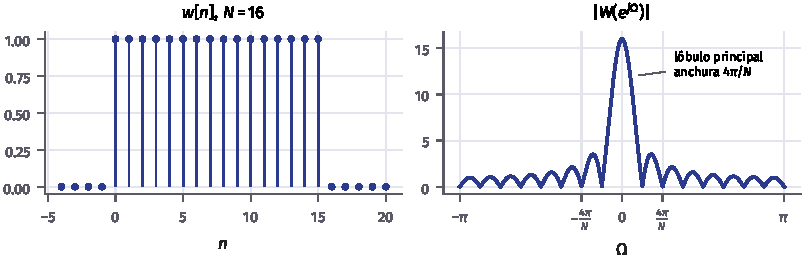
\includegraphics[width=0.85\linewidth]{ventana_rect}
  \caption{Ventana rectangular de $N=16$ muestras y módulo de su DTFT.}
  \label{fig:ventana-rect}
\end{figure}

Un producto en el tiempo es una convolución periódica en frecuencia:

\begin{propiedad}{Efecto del truncamiento}{truncamiento}
  Si $x_N[n]=x[n]\,w[n]$,
  \[
    X_N(\e^{j\Omega})=\frac1{2\pi}\int_0^{2\pi}X(\e^{j\theta})\,W\big(\e^{j(\Omega-\theta)}\big)\dd\theta.
  \]
\end{propiedad}

Cada componente del espectro se sustituye por una copia de $W$. Por ejemplo, la DTFT de $\cos(\Omega_0n)$ son dos impulsos en $\pm\Omega_0$; la del coseno truncado son dos copias de $W$ centradas en $\pm\Omega_0$ (\cref{fig:truncamiento}). El truncamiento tiene dos efectos: \emph{emborrona} el espectro, porque una línea se convierte en un lóbulo de anchura $4\pi/N$, y lo \emph{contamina}, porque los lóbulos secundarios reparten energía por todas las frecuencias. Los dos disminuyen al aumentar $N$, y la \cref{sec:espectral} muestra cómo controlarlos con otras ventanas.

\begin{figure}[ht]
  \centering
  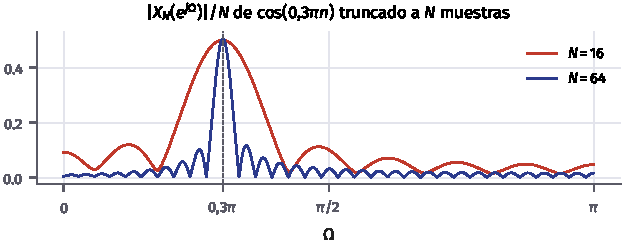
\includegraphics[width=0.65\linewidth]{truncamiento}
  \caption{DTFT de un coseno truncado a $N=16$ y $N=64$ muestras.}
  \label{fig:truncamiento}
\end{figure}

\subsection{Muestrear la DTFT}

El segundo paso es quedarnos con $N$ valores de $X_N(\e^{j\Omega})$. Como es periódica, basta muestrear un periodo, $[0,2\pi)$, en $N$ puntos equiespaciados:
\[
  \Omega_k=\frac{2\pi}{N}k,\qquad k=0,1,\dots,N-1,
\]
separados $\Delta\Omega=2\pi/N$. Si la secuencia solo es no nula en $0\le n<N$,
\[
  X[k]=X(\e^{j\Omega})\big|_{\Omega=2\pi k/N}=\sum_{n=0}^{N-1}x[n]\,\e^{-j\frac{2\pi}{N}kn}.
\]
Esta es la DFT. La \cref{fig:dtft-dft} muestra la DTFT de una secuencia de 5 muestras y sus muestras con $N=8$ y $N=16$: con más muestras se aprecia mejor la forma de la DTFT, pero la información es la misma, porque la secuencia es la misma.

\begin{figure}[ht]
  \centering
  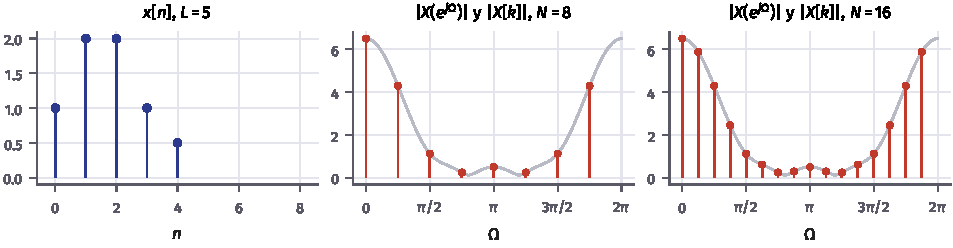
\includegraphics[width=\linewidth]{dtft_dft}
  \caption{Una secuencia de longitud 5, su DTFT y la DFT de 8 y 16 puntos (rellenando con ceros).}
  \label{fig:dtft-dft}
\end{figure}

% =====================================================================
\section{La transformada discreta de Fourier}\label{sec:dft}

\begin{definicion}{DFT e IDFT}{dft}
  La DFT de $N$ puntos de una secuencia $x[n]$, $n=0,\dots,N-1$, es
  \[
    X[k]=\sum_{n=0}^{N-1}x[n]\,W_N^{kn},\qquad k=0,\dots,N-1,
  \]
  con $W_N=\e^{-j2\pi/N}$. La transformada inversa (IDFT) es
  \[
    x[n]=\frac1N\sum_{k=0}^{N-1}X[k]\,W_N^{-kn},\qquad n=0,\dots,N-1.
  \]
\end{definicion}

La IDFT suma sobre $k$, lleva el factor $1/N$ y tiene el signo del exponente cambiado. Para comprobar que invierte la DFT basta la ortogonalidad de las exponenciales discretas:
\begin{equation}\label{eq:ortogonalidad}
  \frac1N\sum_{k=0}^{N-1}W_N^{k(m-n)}=\begin{cases}1 & m-n=0,\pm N,\pm2N,\dots\\0&\text{en otro caso}\end{cases}
\end{equation}
que es una suma geométrica de razón $W_N^{m-n}$: vale $N$ si la razón es 1 y $\frac{1-W_N^{N(m-n)}}{1-W_N^{m-n}}=0$ si no. Sustituyendo la DFT en la IDFT,
\[
  \frac1N\sum_kX[k]W_N^{-kn}=\sum_mx[m]\,\frac1N\sum_kW_N^{k(m-n)}=x[n].
\]

El factor $W_N$ es una raíz $N$-ésima de la unidad, y sus propiedades son la base de la FFT:
\[
  W_N^N=1,\qquad W_N^{k+N}=W_N^k,\qquad W_N^{N/2}=-1,\qquad W_N^{k+N/2}=-W_N^k,\qquad W_N^2=W_{N/2}.
\]

\subsection{Forma matricial}

La DFT es una transformación lineal de $\C^N$ en $\C^N$: $\mathbf X=\mathbf W_N\mathbf x$, con $(\mathbf W_N)_{kn}=W_N^{kn}$:
\[
  \begin{pmatrix}X[0]\\X[1]\\\vdots\\X[N-1]\end{pmatrix}=
  \begin{pmatrix}
    1&1&\cdots&1\\
    1&W_N&\cdots&W_N^{N-1}\\
    \vdots&\vdots&\ddots&\vdots\\
    1&W_N^{N-1}&\cdots&W_N^{(N-1)(N-1)}
  \end{pmatrix}
  \begin{pmatrix}x[0]\\x[1]\\\vdots\\x[N-1]\end{pmatrix}.
\]
La matriz es simétrica y, por \eqref{eq:ortogonalidad}, $\mathbf W_N^*\mathbf W_N=N\mathbf I$: sus columnas son ortogonales y la inversa es $\mathbf W_N^{-1}=\frac1N\mathbf W_N^*$. Calcular el producto directamente cuesta $N^2$ productos complejos; la FFT de la \cref{sec:fft} lo reduce a unos $\frac N2\log_2N$.

\begin{ejemplo}{DFT de cuatro puntos}{dft4}
  Con $N=4$, $W_4=\e^{-j\pi/2}=-j$ y
  \[
    \mathbf W_4=\begin{pmatrix}1&1&1&1\\1&-j&-1&j\\1&-1&1&-1\\1&j&-1&-j\end{pmatrix}.
  \]
  Para $x=(1,3,4,0)$: $X[0]=8$, $X[1]=1-3j-4=-3-3j$, $X[2]=1-3+4=2$ y $X[3]=1+3j-4=-3+3j$. $X[0]$ es la suma de las muestras (la componente continua multiplicada por $N$), y $X[3]=X^*[1]$ porque la secuencia es real.
\end{ejemplo}

\begin{encodigo}
  La DFT del ejemplo~\ref{ej:dft4} como producto de matrices, su comparación con \texttt{fft} y la IDFT con $\frac1N\mathbf W_N^*$.
  \codigo{dft_directa}
\end{encodigo}

\subsection{Extensión periódica y aliasing temporal}

¿Qué ocurre si $x[n]$ es más larga que $N$, o infinita? Las muestras de la DTFT siguen estando definidas, pero agrupando la suma en bloques de $N$ y usando que $W_N^{k(n-mN)}=W_N^{kn}$,
\[
  X(\e^{j2\pi k/N})=\sum_{n=-\infty}^{\infty}x[n]W_N^{kn}=\sum_{n=0}^{N-1}\Big[\sum_{m=-\infty}^{\infty}x[n-mN]\Big]W_N^{kn}.
\]
La IDFT de esas $N$ muestras no devuelve $x[n]$, sino un periodo de su \emph{extensión periódica}.

\begin{propiedad}{Muestreo en frecuencia}{muestreo-frecuencia}
  La IDFT de $N$ muestras equiespaciadas de $\Xd$ es, para $0\le n<N$,
  \[
    \tilde x[n]=\sum_{m=-\infty}^{\infty}x[n-mN].
  \]
  Si $x[n]$ tiene longitud finita $L$ y $N\ge L$, $\tilde x[n]=x[n]$ en $0\le n<N$ y la secuencia se recupera exactamente.
\end{propiedad}

Es el dual del teorema del muestreo: muestrear en el tiempo periodiza el espectro, y muestrear el espectro periodiza la secuencia. Si $N<L$, las copias desplazadas se solapan y se suman: es el \emph{aliasing temporal} (\cref{fig:extension}).

\begin{figure}[ht]
  \centering
  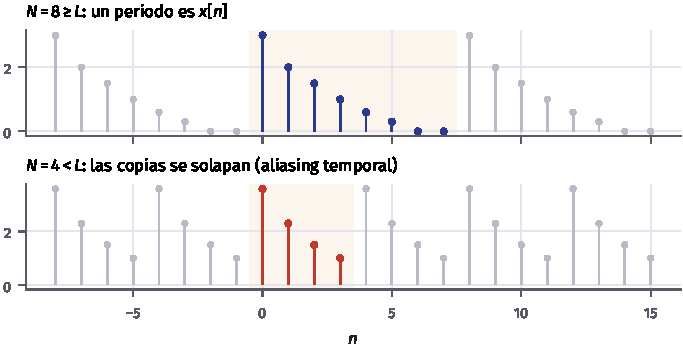
\includegraphics[width=0.75\linewidth]{extension_periodica}
  \caption{Extensión periódica de una secuencia de longitud 6 con $N=8$ y con $N=4$.}
  \label{fig:extension}
\end{figure}

\begin{ejemplo}{Aliasing temporal de una exponencial}{alias-temporal}
  $x[n]=a^nu[n]$ con $\abs a<1$ tiene $\Xd=1/(1-a\e^{-j\Omega})$. Muestreando en $N$ puntos, $X[k]=1/(1-aW_N^k)$, y la IDFT da
  \[
    \tilde x[n]=\sum_{m\ge0}a^{n+mN}=\frac{a^n}{1-a^N},\qquad 0\le n<N.
  \]
  Con $a=0{,}5$ y $N=4$, $\tilde x=(1{,}067;\ 0{,}533;\ 0{,}267;\ 0{,}133)$ en lugar de $(1;\ 0{,}5;\ 0{,}25;\ 0{,}125)$. El error es del orden de $a^N$ y desaparece al aumentar $N$.
\end{ejemplo}

\subsection{Relación con la serie de Fourier discreta}

Una secuencia periódica de periodo $N$ se desarrolla en serie de Fourier discreta (Tema~1):
\[
  \tilde x[n]=\sum_{k=0}^{N-1}c_k\,\e^{j\frac{2\pi}{N}kn},\qquad c_k=\frac1N\sum_{n=0}^{N-1}\tilde x[n]\,\e^{-j\frac{2\pi}{N}kn}.
\]
Comparando con la DFT de un periodo, $X[k]=N\,c_k$. La DFT trata la secuencia como \emph{un periodo de una señal periódica}. Esta interpretación es la clave para entender sus propiedades: un desplazamiento saca muestras por un extremo y las mete por el otro, y la convolución que corresponde al producto de DFT es circular. Por eso los índices se entienden siempre módulo $N$, y escribiremos
\[
  ((n))_N=n\bmod N\in\{0,\dots,N-1\}.
\]

\subsection{Relación con la transformada Z}

Como $\Xd=X(z)|_{z=\e^{j\Omega}}$, la DFT son $N$ muestras de la transformada Z en puntos equiespaciados de la circunferencia unidad, $z_k=\e^{j2\pi k/N}=W_N^{-k}$. Recíprocamente, si $x[n]$ tiene longitud $\le N$, las $N$ muestras determinan $X(z)$ en todo el plano:
\[
  X(z)=\sum_{n=0}^{N-1}\Big[\frac1N\sum_kX[k]W_N^{-kn}\Big]z^{-n}
  =\frac{1-z^{-N}}{N}\sum_{k=0}^{N-1}\frac{X[k]}{1-W_N^{-k}z^{-1}},
\]
sumando la serie geométrica en $n$. Esta fórmula es la base de los filtros diseñados por muestreo en frecuencia (Tema~4).

\begin{flushright}\small\color{pdsgris}Ejercicios 1–4. \herramienta{T3-dft, T3-extension-periodica}.\end{flushright}

% =====================================================================
\section{Propiedades de la DFT}\label{sec:propiedades}

Escribimos $x[n]\overset{\DFT_N}{\longleftrightarrow}X[k]$. Si dos secuencias tienen longitudes distintas, se completa la más corta con ceros hasta $N$; la DFT de $N$ puntos de una secuencia de longitud $L<N$ son $N$ muestras de su DTFT (\emph{relleno con ceros}). Las propiedades se demuestran directamente de la definición, y son las de la DTFT con los desplazamientos y las convoluciones convertidos en circulares. El \cref{tab:propiedades} las resume.

\subsection{Linealidad y desplazamientos circulares}

La DFT es lineal: $a\,x_1[n]+b\,x_2[n]\leftrightarrow a\,X_1[k]+b\,X_2[k]$, siempre que las dos se calculen con la misma $N$. Tanto $X[k]$ como la secuencia que devuelve la IDFT son periódicas de periodo $N$.

\begin{propiedad}{Desplazamiento circular}{desplazamiento}
  \[
    x[((n-m))_N]\longleftrightarrow W_N^{km}X[k],\qquad W_N^{-ln}x[n]\longleftrightarrow X[((k-l))_N].
  \]
\end{propiedad}

Para demostrar la primera, se sustituye $r=((n-m))_N$ en la definición: como $W_N^{kn}=W_N^{k(r+m)}$ (la periodicidad absorbe el módulo), $\sum_nx[((n-m))_N]W_N^{kn}=W_N^{km}\sum_rx[r]W_N^{kr}$. El desplazamiento circular es un desplazamiento de la extensión periódica visto en un periodo: lo que sale por un extremo entra por el otro (\cref{fig:desplazamiento}). Como caso particular de la segunda, con $N$ par, $(-1)^nx[n]=W_N^{-nN/2}x[n]\leftrightarrow X[((k-N/2))_N]$: multiplicar por $(-1)^n$ intercambia las frecuencias bajas y las altas.

\begin{figure}[ht]
  \centering
  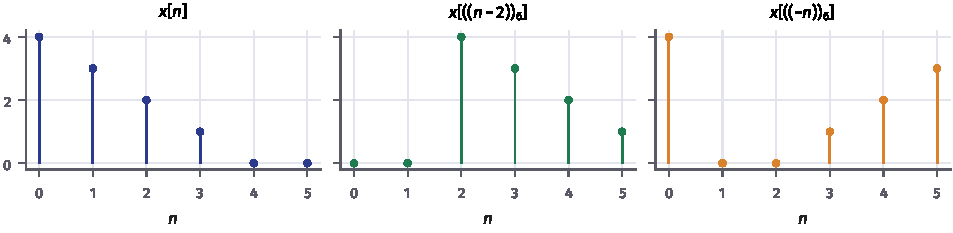
\includegraphics[width=\linewidth]{desplazamiento_circular}
  \caption{Una secuencia, su desplazamiento circular y su inversión circular con $N=6$.}
  \label{fig:desplazamiento}
\end{figure}

\subsection{Inversión, conjugación, simetría y dualidad}

La inversión circular $x[((-n))_N]=(x[0],x[N-1],\dots,x[1])$ tiene DFT $X[((-k))_N]$, y la conjugada $x^*[n]$ tiene DFT $X^*[((-k))_N]$. De esta última se deduce la propiedad más usada en la práctica:

\begin{propiedad}{Simetría hermítica}{hermitica}
  Si $x[n]$ es real, $X[k]=X^*[((-k))_N]=X^*[N-k]$. Por tanto, $\abs{X[k]}=\abs{X[N-k]}$ y $\arg X[k]=-\arg X[N-k]$.
\end{propiedad}

Consecuencias (\cref{fig:simetria}):
\begin{itemize}
  \item $X[0]=\sum_nx[n]$ es real y, si $N$ es par, también lo es $X[N/2]=\sum_n(-1)^nx[n]$.
  \item Las muestras $k>N/2$ son el espejo de las $k<N/2$ y corresponden a las frecuencias negativas $\Omega_k-2\pi$. Basta calcular y representar $k=0,\dots,N/2$, que es lo que hacen \texttt{rfft} en Python y la mayoría de los analizadores.
  \item La parte par circular de $x$, $\frac12(x[n]+x[((-n))_N])$, tiene DFT $\Re X[k]$, y la parte impar circular, $j\Im X[k]$. Una secuencia real y par circular tiene una DFT real.
\end{itemize}

\begin{figure}[ht]
  \centering
  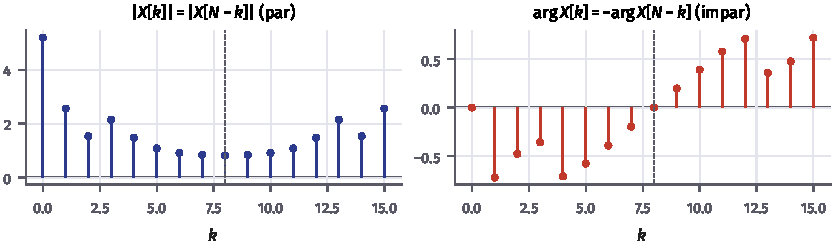
\includegraphics[width=0.8\linewidth]{simetria_dft}
  \caption{Módulo y fase de la DFT de una secuencia real.}
  \label{fig:simetria}
\end{figure}

Por último, la \emph{dualidad}: si $x[n]\leftrightarrow X[k]$, la secuencia $X[n]$ tiene DFT $N\,x[((-k))_N]$. Por ejemplo, $\delta[n]\leftrightarrow1$ y, por dualidad, $1\leftrightarrow N\delta[k]$. Combinando con el desplazamiento, una exponencial que da un número entero $k_0$ de vueltas en $N$ muestras ocupa una sola muestra de la DFT:
\[
  \e^{j\frac{2\pi}{N}k_0n}\longleftrightarrow N\,\delta[((k-k_0))_N].
\]

\subsection{Identidad de Parseval}

\begin{propiedad}{Parseval}{parseval}
  \[
    \sum_{n=0}^{N-1}\abs{x[n]}^2=\frac1N\sum_{k=0}^{N-1}\abs{X[k]}^2.
  \]
\end{propiedad}

Se demuestra sustituyendo $x^*[n]=\frac1N\sum_kX^*[k]W_N^{kn}$ en $\sum_nx[n]x^*[n]$ e intercambiando las sumas: $\frac1N\sum_kX^*[k]\sum_nx[n]W_N^{kn}=\frac1N\sum_k\abs{X[k]}^2$. La energía de las $N$ muestras se reparte entre las frecuencias $\Omega_k$, con $\abs{X[k]}^2/N$ en cada una. En la \cref{sec:potencia} usaremos esta identidad para estimar potencias y densidades espectrales.

\subsection{Convolución circular}

\begin{definicion}{Convolución circular}{conv-circular}
  La convolución circular de $N$ puntos de dos secuencias de longitud $N$ es
  \[
    (x_1\cconv{N}x_2)[n]=\sum_{m=0}^{N-1}x_1[m]\,x_2[((n-m))_N],\qquad n=0,\dots,N-1.
  \]
\end{definicion}

\begin{propiedad}{Convolución circular y producto de DFT}{conv}
  \[
    (x_1\cconv{N}x_2)[n]\longleftrightarrow X_1[k]\,X_2[k],\qquad x_1[n]\,x_2[n]\longleftrightarrow\frac1N(X_1\cconv{N}X_2)[k].
  \]
\end{propiedad}

Para demostrarlo, se calcula la IDFT del producto y se usa \eqref{eq:ortogonalidad}:
\[
  \frac1N\sum_{k}X_1[k]X_2[k]W_N^{-kn}
  =\sum_{m=0}^{N-1}x_1[m]\sum_{l=0}^{N-1}x_2[l]\,\frac1N\sum_{k=0}^{N-1}W_N^{-k(n-m-l)}
  =\sum_{m=0}^{N-1}x_1[m]\,x_2[((n-m))_N],
\]
porque la suma interior vale 1 solo cuando $l=((n-m))_N$.

\begin{errata}
  En algunas transparencias antiguas la IDFT aparecía con la suma en $n$ en lugar de en $k$, y en la última línea de esta demostración se intercambiaban los papeles de $n$ y $m$. Las expresiones correctas son las de arriba.
\end{errata}

\subsection{Convolución circular y convolución lineal}\label{sec:lineal}

La respuesta de un sistema LTI es una convolución \emph{lineal}. Si $x[n]$ tiene longitud $L$ y $h[n]$ longitud $M$, $y=x\conv h$ tiene longitud $L+M-1$. Como el producto de DFT es una convolución circular, interesa saber cuándo coinciden. Rellenando las dos secuencias con ceros hasta $N$, la convolución circular es la lineal \emph{plegada} con periodo $N$ (\cref{fig:conv-circular}):
\[
  (x\cconv{N}h)[n]=\sum_{r=-\infty}^{\infty}(x\conv h)[n-rN],\qquad 0\le n<N.
\]

\begin{propiedad}{Convolución lineal con la DFT}{lineal}
  Si $N\ge L+M-1$, la convolución circular de $N$ puntos de $x$ y $h$, rellenadas con ceros, coincide con la convolución lineal:
  \[
    x\conv h=\IDFT_N\big\{\DFT_N\{x\}\cdot\DFT_N\{h\}\big\}.
  \]
\end{propiedad}

\begin{figure}[ht]
  \centering
  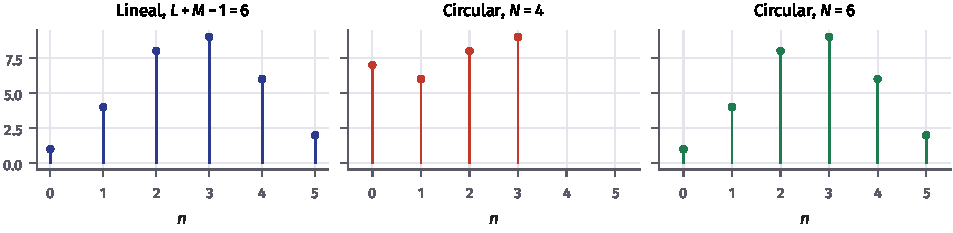
\includegraphics[width=\linewidth]{conv_circular}
  \caption{Convolución lineal de secuencias de longitudes 4 y 3, y convoluciones circulares de 4 y 6 puntos.}
  \label{fig:conv-circular}
\end{figure}

Si $N<L+M-1$, las muestras finales de la convolución lineal se suman a las primeras. Concretamente, si $L\le N<L+M-1$, solo se contaminan las $M-1$ primeras muestras; las restantes son correctas. Esta observación es la base del método de solapamiento y almacenamiento (\cref{sec:bloques}).

\begin{ejemplo}{Respuesta de un FIR con la DFT}{fir}
  Sean $h[n]=(0,2)$ y $x[n]=(1,3,4)$. La convolución lineal es $y[n]=2x[n-1]=(0,2,6,8)$. Con $N=L+M-1=4$:
  \[
    X=(8,\ -3-3j,\ 2,\ -3+3j),\quad H=(2,\ -2j,\ -2,\ 2j),\quad Y=HX=(16,\ -6+6j,\ -4,\ -6-6j),
  \]
  y la IDFT de $Y$ es $(0,2,6,8)$; por ejemplo, $y[0]=\frac14(16-6+6j-4-6-6j)=0$. Con $N=3$ la muestra $y[3]=8$ se pliega sobre $y[0]$ y se obtiene $(8,2,6)$.
\end{ejemplo}

\begin{encodigo}
  Convolución lineal y convolución circular de 3 y 4 puntos del ejemplo~\ref{ej:fir}.
  \codigo{conv_circular}
\end{encodigo}

\begin{table}[ht]
  \centering
  \renewcommand{\arraystretch}{1.25}
  \begin{tabular}{@{}lll@{}}
    \toprule
    Propiedad & Secuencia & DFT de $N$ puntos\\\midrule
    Linealidad & $a\,x_1[n]+b\,x_2[n]$ & $a\,X_1[k]+b\,X_2[k]$\\
    Desplazamiento circular & $x[((n-m))_N]$ & $W_N^{km}X[k]$\\
    Modulación & $W_N^{-ln}x[n]$ & $X[((k-l))_N]$\\
    Inversión circular & $x[((-n))_N]$ & $X[((-k))_N]$\\
    Conjugación & $x^*[n]$ & $X^*[((-k))_N]$\\
    Señal real & $x[n]\in\R$ & $X[k]=X^*[N-k]$\\
    Parte par / impar (señal real) & $x_e[n]$, $x_o[n]$ & $\Re X[k]$, $j\Im X[k]$\\
    Dualidad & $X[n]$ & $N\,x[((-k))_N]$\\
    Convolución circular & $(x_1\cconv{N}x_2)[n]$ & $X_1[k]\,X_2[k]$\\
    Producto & $x_1[n]\,x_2[n]$ & $\frac1N(X_1\cconv{N}X_2)[k]$\\
    Parseval & $\sum_n\abs{x[n]}^2$ & $\frac1N\sum_k\abs{X[k]}^2$\\\bottomrule
  \end{tabular}
  \caption{Propiedades de la DFT.}
  \label{tab:propiedades}
\end{table}

\begin{flushright}\small\color{pdsgris}Ejercicios 5–9. \herramienta{T3-editor-dft, T3-propiedades-dft, T3-convolucion-circular}.\end{flushright}

% =====================================================================
\section{Análisis espectral con la DFT}\label{sec:espectral}

El uso más frecuente de la DFT es estimar el contenido en frecuencia de una señal muestreada. Para hacerlo bien hay que saber leer el eje de frecuencias, entender qué hace el truncamiento y escalar correctamente amplitudes y potencias.

\subsection{Eje de frecuencias}

Si $x[n]=x(nT_s)$, la muestra $k$ de la DFT corresponde a la frecuencia discreta $\Omega_k=2\pi k/N$ y, por $\Omega=\omega T_s$ (Tema~2), a
\[
  f_k=\frac{k}{N}f_s\ \text{Hz},\qquad \omega_k=\frac{2\pi k}{NT_s}\ \text{rad/s}.
\]
La separación entre muestras es
\[
  \Delta f=\frac{f_s}{N}=\frac{1}{NT_s}=\frac{1}{T_{\text{obs}}},
\]
el inverso de la duración del registro. Las muestras $k=0,\dots,N/2$ cubren de 0 a $f_s/2$; las $k>N/2$ corresponden a frecuencias negativas, $f_k-f_s$. Para dibujar el espectro centrado en $[-f_s/2,f_s/2)$ se reordena con \texttt{fftshift} (\cref{fig:ejes}).

\begin{figure}[ht]
  \centering
  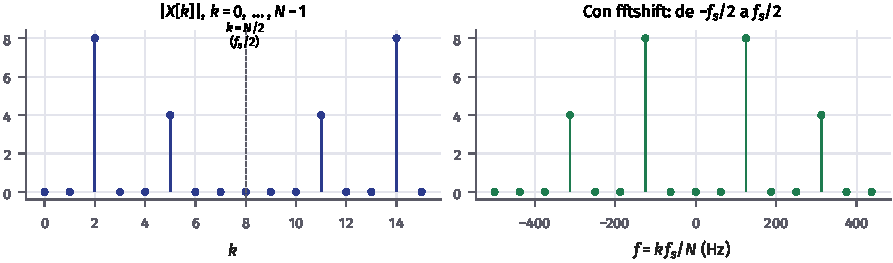
\includegraphics[width=0.9\linewidth]{ejes_dft}
  \caption{DFT de 16 puntos de dos tonos de 125 y 312,5\,Hz muestreados a 1\,kHz, frente a $k$ y frente a la frecuencia.}
  \label{fig:ejes}
\end{figure}

\subsection{Amplitud de una sinusoide}

Si $x[n]=A\cos(\Omega_0n+\phi)$ y $\Omega_0=2\pi k_0/N$, la ventana contiene un número entero de periodos y, por la dualidad,
\[
  X[k_0]=\frac{AN}2\e^{j\phi},\qquad X[N-k_0]=\frac{AN}2\e^{-j\phi},
\]
con el resto de las muestras nulas. La amplitud se lee como $A=2\abs{X[k_0]}/N$ y la fase como $\arg X[k_0]$; la componente continua es $X[0]/N$ (sin el factor 2). Si $\Omega_0$ cae entre dos muestras, la amplitud se reparte entre varias: es la fuga espectral.

\subsection{Fuga espectral}

La DFT muestrea la DTFT de la señal \emph{truncada}, que es la convolución del espectro real con $W(\e^{j\Omega})$ (propiedad~\ref{prop:truncamiento}). Cuando $\Omega_0=2\pi k_0/N$, las demás muestras caen exactamente en los ceros de $W$ y la fuga no se ve. Cuando no, aparecen valores en todas las muestras, y el pico es menor que $AN/2$ (\cref{fig:fuga}). En el peor caso, a media muestra, la pérdida es de $3{,}9$\,dB con la ventana rectangular. Con datos reales casi nunca hay un número entero de periodos en la ventana: la fuga es la norma.

\begin{figure}[ht]
  \centering
  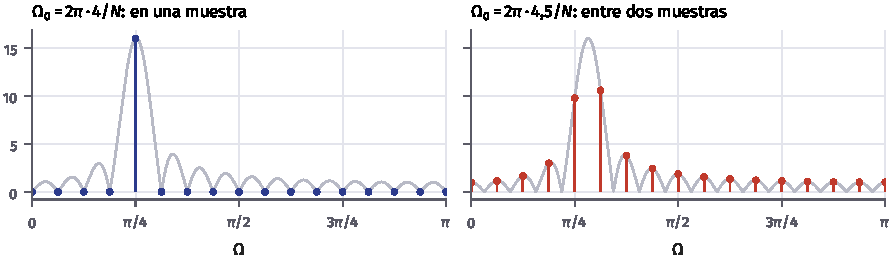
\includegraphics[width=0.9\linewidth]{fuga_espectral}
  \caption{DFT de un coseno con un número entero de periodos en la ventana (izquierda) y con un número no entero (derecha).}
  \label{fig:fuga}
\end{figure}

\subsection{Ventanas}

Para reducir la fuga se multiplica la señal por una ventana $w[n]$ que va suavemente a cero en los extremos, y se calcula la DFT de $x[n]w[n]$. Las más usadas son
\[
  w[n]=a_0-a_1\cos\frac{2\pi n}{N-1}+a_2\cos\frac{4\pi n}{N-1},\qquad 0\le n<N,
\]
con $(a_0,a_1,a_2)=(0{,}5;\ 0{,}5;\ 0)$ para Hann, $(0{,}54;\ 0{,}46;\ 0)$ para Hamming y $(0{,}42;\ 0{,}5;\ 0{,}08)$ para Blackman. Todas tienen lóbulos secundarios mucho más bajos que la rectangular, a cambio de un lóbulo principal más ancho (\cref{fig:ventanas} y \cref{tab:ventanas}).

\begin{figure}[ht]
  \centering
  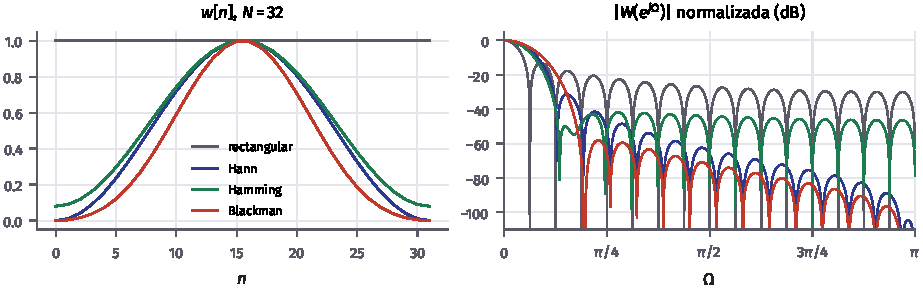
\includegraphics[width=0.95\linewidth]{ventanas}
  \caption{Ventanas de 32 muestras y módulo normalizado de su DTFT en decibelios.}
  \label{fig:ventanas}
\end{figure}

\begin{table}[ht]
  \centering
  \begin{tabular}{@{}lccc@{}}
    \toprule
    Ventana & lóbulo principal & primer lóbulo secundario & pérdida a media muestra\\\midrule
    Rectangular & $4\pi/N$ & $-13$\,dB & $3{,}9$\,dB\\
    Hann & $8\pi/N$ & $-31$\,dB & $1{,}4$\,dB\\
    Hamming & $8\pi/N$ & $-42$\,dB & $1{,}7$\,dB\\
    Blackman & $12\pi/N$ & $-58$\,dB & $1{,}1$\,dB\\\bottomrule
  \end{tabular}
  \caption{Características de las ventanas más comunes (anchura del lóbulo principal entre ceros).}
  \label{tab:ventanas}
\end{table}

La ventana cambia la escala: para una sinusoide en una muestra, $\abs{X_w[k_0]}=\frac A2\sum_nw[n]$, así que la amplitud se lee como $A=2\abs{X_w[k_0]}/\sum_nw[n]$. La \cref{fig:tonos} muestra para qué sirve una buena ventana: un tono 40\,dB más débil que otro, a 80\,Hz de distancia, queda oculto por la fuga de la ventana rectangular y se ve claramente con Hann o Blackman. Como regla práctica, Hann es una buena elección general; la rectangular solo conviene si la señal contiene un número entero de periodos o es un transitorio que cabe entero en la ventana.

\begin{figure}[ht]
  \centering
  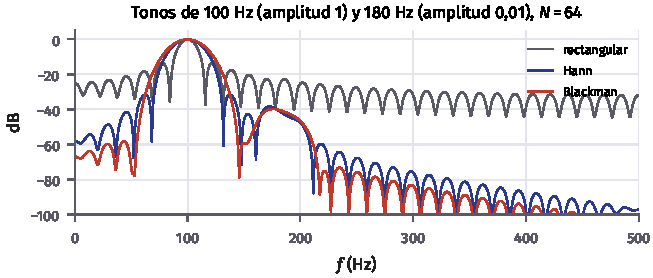
\includegraphics[width=0.7\linewidth]{ventana_tonos}
  \caption{Espectro de dos tonos de amplitudes 1 y 0,01 con tres ventanas.}
  \label{fig:tonos}
\end{figure}

\begin{encodigo}
  Espectro de amplitud de dos tonos con ventana de Hann. Con $N=200$ a 1\,kHz, $\Delta f=5$\,Hz: el tono de 152\,Hz cae entre dos muestras, pero la ventana limita la fuga.
  \codigo{espectro_dft}
\end{encodigo}

\subsection{Resolución y relleno con ceros}

Dos tonos se distinguen si sus lóbulos principales no se funden. Con la ventana rectangular, el lóbulo tiene semianchura $2\pi/N$, es decir, $f_s/N$ en hercios, y la condición aproximada es
\[
  \abs{f_2-f_1}\gtrsim\frac{f_s}{N}=\frac{1}{T_{\text{obs}}};
\]
con Hann o Hamming hace falta aproximadamente el doble. La resolución en frecuencia está fijada por la \emph{duración del registro}, no por la frecuencia de muestreo.

Rellenar la secuencia con ceros hasta $N'>N$ y calcular la DFT de $N'$ puntos da más muestras de la misma DTFT: interpola el espectro y facilita localizar los picos, pero \emph{no mejora la resolución}, porque no añade información (\cref{fig:resolucion}). También se rellena con ceros para llegar a una longitud que sea potencia de 2 y la FFT sea más rápida.

\begin{figure}[ht]
  \centering
  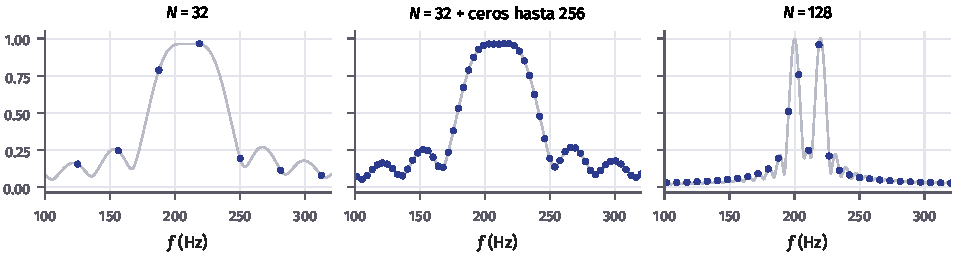
\includegraphics[width=\linewidth]{resolucion}
  \caption{Tonos de 200 y 220\,Hz a $f_s=1$\,kHz: con $N=32$ no se separan, ni siquiera rellenando con ceros; con $N=128$ sí.}
  \label{fig:resolucion}
\end{figure}

\subsection{Potencia y densidad espectral de potencia}\label{sec:potencia}

Por Parseval, la potencia media de las $N$ muestras se reparte entre las frecuencias:
\[
  P=\frac1N\sum_{n=0}^{N-1}\abs{x[n]}^2=\sum_{k=0}^{N-1}\Big|\frac{X[k]}N\Big|^2.
\]
\begin{itemize}
  \item La \emph{potencia en la muestra $k$} es $\abs{X[k]/N}^2$. Una sinusoide de amplitud $A$ en una muestra aporta $A^2/4$ en $k_0$ y otro tanto en $N-k_0$: en total, $A^2/2$, como debe ser. En decibelios, $P_k=20\log_{10}(\abs{X[k]}/N)$.
  \item La \emph{densidad espectral de potencia} se estima con el \emph{periodograma},
  \[
    \hat\Phi_{xx}(f_k)=\frac{\abs{X[k]}^2}{N\,f_s},
  \]
  en unidades$^2$/Hz, de modo que $\sum_k\hat\Phi_{xx}(f_k)\,\Delta f=P$. En decibelios por hercio, $10\log_{10}\hat\Phi_{xx}$.
\end{itemize}
La diferencia importa con señales de banda ancha. Para un ruido blanco de varianza $\sigma^2$, $E\abs{X[k]}^2=N\sigma^2$: la potencia por muestra, $\sigma^2/N$, baja al aumentar $N$, pero la densidad, $\sigma^2/f_s$, no depende de $N$. Para un tono pasa lo contrario: su potencia está en una muestra y no depende de $N$. Por eso, al aumentar $N$, un tono sobresale más del ruido en la DFT.

Con ventana, la densidad se normaliza con $\sum w^2[n]$ en lugar de $N$: $\hat\Phi_{xx}=\abs{X_w[k]}^2/(f_s\sum_nw^2[n])$. El periodograma de una señal aleatoria fluctúa mucho alrededor de su valor medio y no mejora al aumentar $N$; se reduce la varianza promediando los periodogramas de varios tramos (método de Welch, Tema~6).

\begin{errata}
  En algunas transparencias antiguas se llamaba $\Phi_{xx}$ en dB a la potencia por muestra $20\log_{10}(\abs{X[k]}/N)$, y la autocorrelación aparecía sin el factor $1/T$ y con $\dd\tau$ en lugar de $\dd t$. Las definiciones correctas son las de esta sección y del Tema~6.
\end{errata}

\subsection{Espectrograma}

La DFT de una señal larga mezcla lo que ocurre en todos los instantes: no dice cuándo aparece cada frecuencia. Para señales cuyo contenido cambia con el tiempo (voz, música, vibraciones de una máquina que acelera) se usa la \emph{transformada de Fourier de tiempo corto} (STFT), que calcula la DFT de tramos sucesivos con ventana:
\[
  X_m[k]=\sum_{n=0}^{N_w-1}x[n+mR]\,w[n]\,W_{N_w}^{kn}.
\]
$N_w$ es la longitud de los tramos y $R$ el paso entre tramos; con $R<N_w$ se solapan, y lo habitual es un solape del 50 al 75\,\%. El \emph{espectrograma} es la imagen de $\abs{X_m[k]}^2$, con el tiempo $mRT_s$ en abscisas y la frecuencia $kf_s/N_w$ en ordenadas (\cref{fig:espectrograma}).

La elección de $N_w$ es un compromiso: tramos largos dan buena resolución en frecuencia ($\Delta f=f_s/N_w$) pero mala en el tiempo, y tramos cortos al revés. No es una limitación del método sino del propio concepto de «frecuencia en un instante».

\begin{figure}[ht]
  \centering
  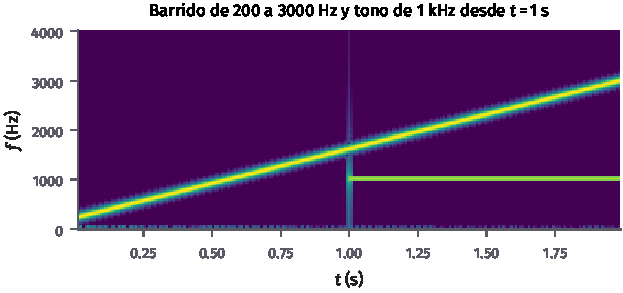
\includegraphics[width=0.7\linewidth]{espectrograma}
  \caption{Espectrograma de un barrido de frecuencia y de un tono que empieza en $t=1$\,s ($N_w=256$, solape del 75\,\%).}
  \label{fig:espectrograma}
\end{figure}

\begin{encodigo}
  STFT calculada a mano, tramo a tramo. \texttt{scipy.signal.spectrogram} y \texttt{spectrogram} de Matlab hacen lo mismo con más opciones.
  \codigo{espectrograma}
\end{encodigo}

\begin{flushright}\small\color{pdsgris}Ejercicios 10–13. \herramienta{T3-dft, T3-ventanas}.\end{flushright}

% =====================================================================
\section{FFT y convolución rápida}\label{sec:fft}

\subsection{Coste de la DFT directa}

Calcular las $N$ muestras de la DFT con la definición cuesta $N^2$ productos complejos y $N(N-1)$ sumas. Con $N=1024$ es un millón de productos por espectro. La \emph{transformada rápida de Fourier} (FFT) es una familia de algoritmos que calculan exactamente la misma DFT con un número de operaciones proporcional a $N\log_2N$. Su publicación por Cooley y Tukey en 1965 hizo práctico el procesado digital de señales; más tarde se descubrió que Gauss había usado la misma idea hacia 1805 para interpolar órbitas de asteroides.

\subsection{Diezmado en el tiempo en base 2}

Sea $N=2^p$. Separamos las muestras de índice par, $n=2r$, y las de índice impar, $n=2r+1$:
\[
  X[k]=\sum_{r=0}^{N/2-1}x[2r]\,W_N^{2rk}+\sum_{r=0}^{N/2-1}x[2r+1]\,W_N^{(2r+1)k}.
\]
Como $W_N^2=W_{N/2}$,
\[
  X[k]=\underbrace{\sum_{r=0}^{N/2-1}x[2r]\,W_{N/2}^{rk}}_{F[k]}+W_N^k\underbrace{\sum_{r=0}^{N/2-1}x[2r+1]\,W_{N/2}^{rk}}_{G[k]},\qquad k=0,\dots,N-1,
\]
donde $F[k]$ y $G[k]$ son las DFT de $N/2$ puntos de las muestras pares e impares. Son periódicas de periodo $N/2$, y $W_N^{k+N/2}=-W_N^k$, así que basta calcularlas para $k=0,\dots,N/2-1$:

\begin{propiedad}{Mariposa del diezmado en el tiempo}{mariposa}
  \[
    X[k]=F[k]+W_N^k\,G[k],\qquad X[k+N/2]=F[k]-W_N^k\,G[k],\qquad k=0,\dots,\tfrac N2-1.
  \]
\end{propiedad}

\begin{errata}
  En algunas transparencias antiguas el factor $W_N^k$ aparecía como $W_{N/2}^r$ fuera del sumatorio, y la segunda mitad se escribía para $k=N/2,\dots,N-1$. Las fórmulas correctas son las de arriba: $k$ recorre solo la primera mitad y la segunda se obtiene con el signo cambiado.
\end{errata}

Cada par de salidas cuesta un producto complejo ($W_N^kG[k]$) y dos sumas: es la \emph{mariposa}. Las DFT de $N/2$ puntos se descomponen del mismo modo en DFT de $N/4$, y así hasta DFT de un punto, que son la propia muestra. Hay $\log_2N$ etapas de $N/2$ mariposas, lo que da
\[
  \frac N2\log_2N\ \text{productos complejos}\qquad\text{y}\qquad N\log_2N\ \text{sumas}.
\]
Para $N=1024$ son 5120 productos en lugar de un millón (\cref{fig:complejidad}). Muchos de esos productos son por $W_N^0=1$ o por $W_N^{N/4}=-j$, que no cuestan nada, así que el número real es aún menor.

\begin{figure}[ht]
  \centering
  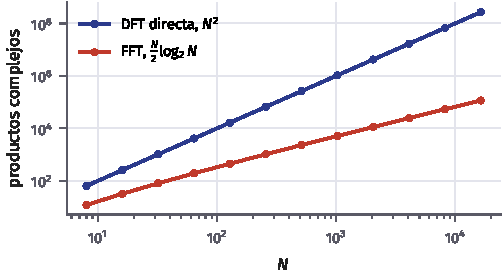
\includegraphics[width=0.5\linewidth]{complejidad}
  \caption{Productos complejos de la DFT directa y de la FFT en base 2.}
  \label{fig:complejidad}
\end{figure}

Al aplicar la separación en pares e impares repetidamente, la entrada queda en \emph{orden de bits invertidos}: la muestra $n$ va a la posición cuyo índice en binario es el de $n$ leído al revés. Con $N=8$, el orden es $x[0],x[4],x[2],x[6],x[1],x[5],x[3],x[7]$.

\begin{ejemplo}{FFT de cuatro puntos}{fft4}
  Para $x=(1,3,4,0)$: las muestras pares son $(1,4)$, con DFT $F=(5,-3)$; las impares, $(3,0)$, con $G=(3,3)$. Con $W_4^0=1$ y $W_4^1=-j$:
  \[
    X[0]=5+3=8,\quad X[1]=-3-3j,\quad X[2]=5-3=2,\quad X[3]=-3+3j,
  \]
  como en el ejemplo~\ref{ej:dft4}, con 4 productos (dos de ellos triviales) en lugar de 16.
\end{ejemplo}

\begin{encodigo}
  FFT iterativa en base 2: reordenación por inversión de bits y $\log_2N$ etapas de mariposas.
  \codigo{fft_radix2}
\end{encodigo}

\subsection{Otras variantes}

El \emph{diezmado en frecuencia} separa las muestras pares e impares de $X[k]$ en lugar de las de $x[n]$, y deja la salida en orden de bits invertidos. Hay algoritmos en base 4 y de base mixta, y otros para cualquier $N$, incluso primo (Rader, Bluestein). Las bibliotecas actuales, como FFTW (la que usa Matlab) o la de NumPy, eligen el algoritmo según $N$; son más rápidas cuando $N$ es potencia de 2 o tiene factores pequeños. La IFFT no necesita un algoritmo propio:
\[
  x[n]=\frac1N\Big(\sum_kX^*[k]W_N^{kn}\Big)^*=\frac1N\big(\operatorname{FFT}\{X^*\}\big)^*,
\]
y con señales reales se aprovecha la simetría hermítica para hacer la mitad de trabajo (\texttt{rfft}).

\subsection{Convolución rápida}

Por la propiedad~\ref{prop:lineal}, la convolución lineal de $x$ (longitud $L$) y $h$ (longitud $M$) se puede calcular rellenando ambas con ceros hasta $N\ge L+M-1$, multiplicando sus FFT y calculando la IFFT. El coste es de tres FFT y $N$ productos, unos $\frac32N\log_2N+N$ productos complejos, frente a los $LM$ de la suma directa. Con $L=M=1000$ y $N=2048$, unos $3{,}6\cdot10^4$ frente a $10^6$. Para filtros muy cortos (unas decenas de coeficientes) la suma directa sigue siendo competitiva, sobre todo en un DSP con instrucciones de multiplicar y acumular. Si se filtran muchas señales con el mismo $h$, $H[k]$ se calcula una sola vez.

\subsection{Señales largas: procesado por bloques}\label{sec:bloques}

Si la entrada es muy larga o no termina (audio en tiempo real), no se puede esperar a tenerla entera. Se divide en bloques y se combinan los resultados.

\paragraph{Solapamiento y suma (\emph{overlap-add}).} Se divide la entrada en bloques de $L$ muestras, $x[n]=\sum_ix_i[n-iL]$. Por linealidad, $y=\sum_i(x_i\conv h)[n-iL]$. Cada $x_i\conv h$ se calcula por FFT de $N\ge L+M-1$ puntos y tiene $L+M-1$ muestras, así que las salidas de bloques consecutivos se solapan en $M-1$ muestras, que se suman (\cref{fig:ola}).

\begin{figure}[ht]
  \centering
  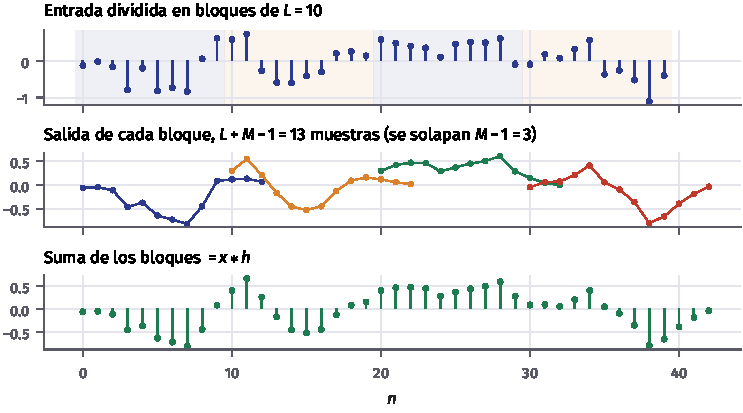
\includegraphics[width=0.8\linewidth]{solapamiento_suma}
  \caption{Solapamiento y suma con bloques de 10 muestras y un filtro de 4 coeficientes.}
  \label{fig:ola}
\end{figure}

\paragraph{Solapamiento y almacenamiento (\emph{overlap-save}).} Se toman bloques de entrada de $N$ muestras que se solapan $M-1$ con el anterior, y se calcula su convolución \emph{circular} de $N$ puntos con $h$. Según la \cref{sec:lineal}, las $M-1$ primeras muestras están contaminadas por el plegado circular y se descartan; las $N-M+1$ restantes coinciden con la convolución lineal y se guardan.

Los dos métodos dan el mismo resultado con un coste parecido, y el retardo es de un bloque. Los implementan \texttt{oaconvolve} (de \texttt{scipy.signal}) y \texttt{fftfilt} (de Matlab).

\begin{encodigo}
  Solapamiento y suma con bloques de 226 muestras, un FIR de 31 coeficientes y FFT de $N=256$. El resultado coincide con la convolución directa.
  \codigo{solapamiento_suma}
\end{encodigo}

\subsection{Sistemas IIR}

Si $h[n]$ tiene duración infinita, las muestras $H[k]=H(\e^{j2\pi k/N})$ existen, pero su IDFT es la extensión periódica $h_N[n]=\sum_rh[n-rN]$ (propiedad~\ref{prop:muestreo-frecuencia}). Para $h[n]=a^nu[n]$ es $h_N[n]=a^n/(1-a^N)$ (ejemplo~\ref{ej:alias-temporal}), y la DFT filtra con un error del orden de $a^N$ (\cref{fig:iir}). Con $N$ suficientemente grande el error es despreciable, y por eso el filtrado en frecuencia con la FFT se usa también con sistemas IIR o con respuestas medidas, que son largas. Pero lo exacto, y normalmente mucho más barato, es implementar el sistema con su ecuación en diferencias (Tema~4).

\begin{errata}[Errata de versiones anteriores]
  Algunas transparencias antiguas afirmaban que la DFT no se puede usar con sistemas IIR ni con entradas de duración infinita. Con entradas largas se usa el procesado por bloques; con sistemas IIR, la DFT da una aproximación cuyo error se controla con $N$.
\end{errata}

\begin{figure}[ht]
  \centering
  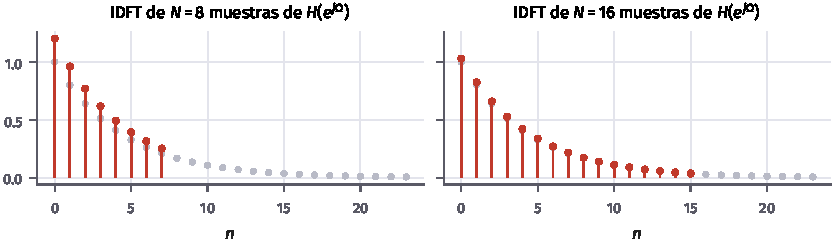
\includegraphics[width=0.8\linewidth]{muestreo_frecuencia}
  \caption{IDFT de 8 y 16 muestras de $H(\e^{j\Omega})=1/(1-0{,}8\e^{-j\Omega})$ frente a $h[n]=0{,}8^nu[n]$.}
  \label{fig:iir}
\end{figure}

\begin{flushright}\small\color{pdsgris}Ejercicios 14–16. \herramienta{T3-fft-mariposa, T3-solapamiento-suma}.\end{flushright}

% =====================================================================
\section*{Resumen del tema}
\addcontentsline{toc}{section}{Resumen del tema}

\begin{itemize}
  \item Observar $N$ muestras es enventanar: el espectro se convoluciona con $W(\e^{j\Omega})$, de lóbulo principal $4\pi/N$.
  \item DFT: $X[k]=\sum_{n=0}^{N-1}x[n]W_N^{kn}$; IDFT: $x[n]=\frac1N\sum_{k=0}^{N-1}X[k]W_N^{-kn}$; $W_N=\e^{-j2\pi/N}$. $X[k]$ es la DTFT en $2\pi k/N$.
  \item Muestrear en frecuencia periodiza en el tiempo; sin aliasing temporal si $N\ge L$. $X[k]=Nc_k$ y los índices se toman módulo $N$.
  \item Propiedades circulares; señal real: $X[k]=X^*[N-k]$; Parseval: $\sum\abs x^2=\frac1N\sum\abs X^2$.
  \item El producto de DFT es una convolución circular, que coincide con la lineal si $N\ge L+M-1$.
  \item $f_k=kf_s/N$, $\Delta f=1/T_{\text{obs}}$; amplitud $2\abs{X[k_0]}/N$; potencia por muestra $\abs{X[k]/N}^2$; periodograma $\abs{X[k]}^2/(Nf_s)$.
  \item Fuga espectral y ventanas: menos fuga a cambio de un lóbulo principal más ancho. El relleno con ceros interpola pero no resuelve.
  \item Espectrograma: DFT de tramos con ventana, con un compromiso entre resolución en tiempo y en frecuencia.
  \item FFT: $X[k]=F[k]+W_N^kG[k]$, $X[k+N/2]=F[k]-W_N^kG[k]$; $\frac N2\log_2N$ productos.
  \item Convolución rápida con FFT; señales largas por solapamiento y suma o almacenamiento.
\end{itemize}

% =====================================================================
\section*{Bibliografía}
\addcontentsline{toc}{section}{Bibliografía}

\begin{itemize}
  \item J.~G. Proakis y D.~G. Manolakis, \emph{Tratamiento digital de señales}, 4.ª ed. Pearson Prentice Hall, 2007. Capítulos 7 (DFT) y 8 (FFT).
  \item A.~V. Oppenheim y R.~W. Schafer, \emph{Tratamiento de señales en tiempo discreto}, 3.ª ed. Pearson, 2011. Capítulos 8 (DFT), 9 (FFT) y 10 (análisis de Fourier con la DFT).
  \item F.~T. Ulaby y A.~E. Yagle, \emph{Signals and Systems: Theory and Applications}, 2.ª ed. Michigan Publishing Services, 2024. Capítulo de señales en tiempo discreto, apartados de DFT y FFT. Descarga libre en\\ \url{https://services.publishing.umich.edu/Books/S/Signals-and-Systems}.
  \item V.~K. Ingle y J.~G. Proakis, \emph{Digital Signal Processing Using MATLAB}, 3.ª ed. Cengage Learning, 2012. Capítulo 5, con ejemplos en Matlab.
  \item F.~J. Harris, «On the use of windows for harmonic analysis with the discrete Fourier transform», \emph{Proceedings of the IEEE}, 66(1), 1978. La referencia clásica sobre ventanas.
\end{itemize}

\end{document}
